\begin{abox}
	Quantum Mechanics
	\end{abox}
\begin{enumerate}
	\item A particle of mass $m$ and energy $E$, moving in the positive $x$ direction, is incident on a step potential at $x=0$, as indicated in the figure. The height of the potential is $V_{0}$, where $V_{0}>E$. At $x=x_{0}$, where $x_{0}>0$, the probability of finding the electron is $\frac{1}{e}$ times the probability of finding it at $x=0$.
	If $\alpha=\sqrt{\frac{2 m\left(V_{0}-E\right)}{\hbar^{2}}}$, the value of $x_{0}$ is
	\begin{figure}[H]
		\centering
		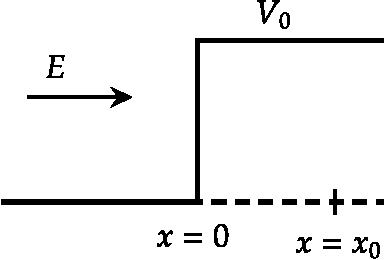
\includegraphics[height=2.3cm,width=4cm]{QM-1}
	\end{figure}
	 \begin{tasks}(2)
		\task[\textbf{a.}]$\frac{2}{\alpha}$
		\task[\textbf{b.}]$\frac{1}{\alpha}$
		\task[\textbf{c.}]$\frac{1}{2 \alpha}$
		\task[\textbf{d.}] $\frac{1}{4 \alpha}$
	\end{tasks}
\begin{answer}
	$$
	\begin{aligned}
	\frac{1}{e}=e^{-2 \alpha x_{0}}=e^{-1}=e^{-2 \alpha x_{0}} \Rightarrow x_{0}=\frac{1}{2 \alpha}
\end{aligned}
$$
So the correct answer is \textbf{Option (c)}
\end{answer}
	\item A free particle of energy $E$, characterized by a plane wave of wavelength $\lambda$ enters a region of constant potential $-V$ (where $E>V>0$ ). Within the region of the potential, the wavelength of the particle is $\frac{\lambda}{2}$. The ratio $\frac{V}{E}$ is:
	 \begin{tasks}(2)
		\task[\textbf{a.}]$\frac{-1}{3}$
		\task[\textbf{b.}] $-3$
		\task[\textbf{c.}] 3
		\task[\textbf{d.}]  $\frac{1}{3}$
	\end{tasks}
\begin{answer}
	$$
	\begin{aligned}
	E&=\frac{P^{2}}{2 m}=\frac{\hbar^{2}}{2 m \lambda^{2}}\\
	\frac{\lambda}{2}&=\sqrt{\frac{\hbar}{2 m(E+V)}}\qquad \lambda^{2}=\frac{\hbar^{2}}{2 m E}\\
	\left(\frac{\lambda}{2}\right)^{2}&=\frac{\hbar^{2}}{2 m(E+V)}\\
	u&=\frac{E+V}{E}=1+\frac{V}{E} \Rightarrow \frac{V}{E}=3
\end{aligned}
$$
So the correct answer is \textbf{Option (c)}
\end{answer}
	\item A particle with energy $E$ is incident on a potential given by
	$$
	V(x)=\left\{\begin{array}{cc}
	0, & x<0 \\
	V_{0}, & x \geq 0
	\end{array}\right.
	$$
	The wave function of the particle for $E<V_{0}$ in the region $x>0$ (in terms of positive constants $A, B$ and $k)$ is
	 \begin{tasks}(2)
		\task[\textbf{a.}] $A e^{k x}+B e^{-k x}$
		\task[\textbf{b.}]$A e^{-k x}$
		\task[\textbf{c.}]$A e^{i k x}+B e^{-i k x}$
		\task[\textbf{d.}] Zero
	\end{tasks}
\begin{answer}
	$$
	\begin{aligned}
	\text { For } &x>0 ;-\frac{\hbar^{2}}{2 m} \frac{d^{2} \psi_{\mathrm{II}}}{d}+V_{0} \psi_{\mathrm{II}}=E \psi_{\mathrm{II}} ; \quad E<V_{0}\\
	\psi_{\mathrm{II}}&=B e^{k x}+A e^{-k x}, \text { where } k=\sqrt{\frac{2 m\left(V_{0}-E\right)}{\hbar^{2}}}\\
	\psi_{\mathrm{II}} &\rightarrow 0 \text { as } x \rightarrow \infty \Rightarrow A=0 \Rightarrow \psi_{\mathrm{II}}=A e^{-k x}
\end{aligned}
$$
So the correct answer is \textbf{Option (b)}
\end{answer}
	\item Consider the motion of a quantum particle of mass $m$ and energy $E$ under the influence of a step potential of height $V_{0}$. If $R$ denotes the reflection coefficient, which one of the following statements is true?
	\begin{figure}[H]
		\centering
		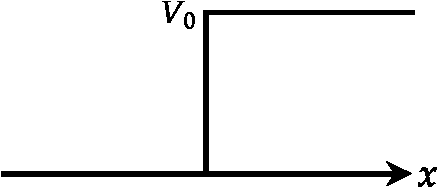
\includegraphics[height=2cm,width=4cm]{QM-2}
	\end{figure}
	 \begin{tasks}(2)
		\task[\textbf{a.}]If $E=\frac{4}{3} V_{0}, R=1$
		\task[\textbf{b.}]$E=\frac{4}{3} V_{0}, R=0$
		\task[\textbf{c.}]$E=\frac{1}{2} V_{0}, R=1$
		\task[\textbf{d.}] $E=\frac{1}{2} V_{0}, R=0.5$
	\end{tasks}
\begin{answer}
	$$
	\begin{aligned}
	E&=\frac{V_{0}}{2} \quad \Rightarrow E<V_{0}\\
	\text { So, }& R=1\\
	&\text { Therefore, option (c) is correct }
\end{aligned}
$$
So the correct answer is \textbf{Option (c)}
\end{answer}
\item Consider a potential barrier $A$ of height $V_{0}$ and width $b$, and another potential barrier $B$ of height $2 V_{0}$ and the same width $b$. The ratio $T_{A} / T_{B}$ of tunnelling probabilities $T_{A}$ and $T_{B}$, through barriers $A$ and $B$ respectively, for a particle of energy $V_{0} / 100$ is best approximated by
 \begin{tasks}(2)
	\task[\textbf{a.}]$\exp \left[(\sqrt{1.99}-\sqrt{0.99}) \sqrt{8 m V_{0} b^{2} / \hbar^{2}}\right]$
	\task[\textbf{b.}]$\exp \left[(\sqrt{1.98}-\sqrt{0.98}) \sqrt{8 m V_{0} b^{2} / \hbar^{2}}\right]$
	\task[\textbf{c.}]$\exp \left[(\sqrt{2.99}-\sqrt{0.99}) \sqrt{8 m V_{0} b^{2} / \hbar^{2}}\right]$
	\task[\textbf{d.}] $\exp \left[(\sqrt{2.98}-\sqrt{0.98}) \sqrt{8 m V_{0} b^{2} / \hbar^{2}}\right]$
\end{tasks}
\begin{answer}
	$$
	\begin{aligned}
	T \alpha e^{-\sqrt{2 m(V-E)}}, &\quad \text { where } E=\frac{V_{0}}{100}\\
	\text { For potential } &A, \quad V=V_{0}\\
	T_{A} \alpha e^{-\sqrt{\frac{2 m}{\hbar^{2}}\left(V_{0}-\frac{V_{0}}{100}\right)}} &\Rightarrow T_{A} \alpha e^{-\sqrt{\frac{2 m}{\hbar^{2}}\left(\frac{99}{100} V_{0}\right)}} \alpha e^{-\sqrt{2 m\left(0.99 V_{0}\right)}}\\
	\text { For Potential } &B, \quad V=2 V_{0} \text { and } E=\frac{V_{0}}{100}\\
	T_{B} \alpha e^{-\sqrt{\frac{2 m}{\hbar^{2}}\left(2 V_{0}-\frac{V_{0}}{100}\right)}} &\Rightarrow T_{B} \alpha e^{-\sqrt{\frac{2 m}{h^{2}}\left(\frac{199 V_{0}}{100}\right)}} \alpha e^{-\sqrt{2 m\left(1.99 V_{0}\right)}}\\
	\frac{T_{A}}{T_{B}}&=\frac{e^{-\sqrt{0.99 V_{0}}}}{e^{-\sqrt{1.99 V_{0}}}}\\
	\frac{T_{A}}{T_{B}}&=\left(e^{\sqrt{1.99 V_{0}}}-e^{-\sqrt{0.99 V_{0}}}\right)
\end{aligned}
$$
So the correct answer is \textbf{Option (a)}
\end{answer}
\item If probability density $\rho(x)=\left\{\begin{array}{c}\exp \left(-\frac{x}{\lambda}\right), x \geq 0 \\ 0, x<0\end{array}\right.$ of a one dimensional system is and then the probability that system has value $x \geq \lambda$ assume $\lambda>0$
 \begin{tasks}(2)
	\task[\textbf{a.}]$\frac{1}{e-1}$
	\task[\textbf{b.}]$\frac{1}{e+1}$
	\task[\textbf{c.}]$\frac{1}{e}$
	\task[\textbf{d.}] $\frac{e-1}{e+1}$ 
\end{tasks}
\begin{answer}
	$$
	\begin{aligned}
	p(x \geq \lambda)=\frac{\int_{\lambda}^{\infty} \exp \left(-\frac{x}{\lambda}\right) d x}{\int_{0}^{\infty} \exp \left(-\frac{x}{\lambda}\right) d x}=\frac{1}{e}
\end{aligned}
$$
So the correct answer is \textbf{Option (c)}
\end{answer}
\item If an operator $A$ is defined as $A\left|\phi_{n}\right\rangle=n a_{0}\left|\phi_{n}\right\rangle n=1,2,3$ where $\left\langle\phi_{m} \mid \phi_{n}\right\rangle=\delta_{m, n}$. If $A$ is measured on state $\left|\psi_{0}\right\rangle=\left(2\left|\phi_{1}\right\rangle-3 i\left|\phi_{2}\right\rangle\right)$ what will average value of measurement of $A$
 \begin{tasks}(2)
	\task[\textbf{a.}]$5 a_{0}$
	\task[\textbf{b.}]$\frac{35 a_{0}}{13}$
	\task[\textbf{c.}]$\frac{3 a_{0}}{5}$
	\task[\textbf{d.}] $\frac{22 a_{0}}{13}$
\end{tasks}
\begin{answer}
	$$
	\begin{aligned}
	&\left|\psi_{0}\right\rangle=\left(2\left|\phi_{1}\right\rangle-3 i\left|\phi_{2}\right\rangle\right), A\left|\phi_{n}\right\rangle=n a_{0}\left|\phi_{n}\right\rangle\\
	&\text { Now measurement of } A \text { on state }\left|\psi_{0}\right\rangle \text { is } a_{0} \text { and } 2 a_{0} \text { with eigen state }\left|\phi_{1}\right\rangle \text { and }\left|\phi_{2}\right\rangle  \text { respectively }\\
	&\text { Probability of measurement of } a_{0} \text { is } P\left(a_{0}\right)=\frac{\left\langle\phi_{1} \mid \psi_{0}\right\rangle}{\left\langle\psi_{0} \mid \psi_{0}\right\rangle}=\frac{4}{13}\\
	&\text { Probability of measurement of } 2 a_{0} \text { is } P\left(2 a_{0}\right)=\frac{\left\langle\phi_{2} \mid \psi_{0}\right\rangle}{\left\langle\psi_{0} \mid \psi_{0}\right\rangle}=\frac{9}{13}\\
	&\text { Average value of measurement of } A \text { is }\\
	&\langle A\rangle=\frac{\left\langle\psi_{0}|A| \psi_{0}\right\rangle}{\left\langle\psi_{0} \mid \psi_{0}\right\rangle}=\sum_{n} a_{n} P\left(a_{n}\right) \Rightarrow a_{0} \times \frac{4}{13}+2 a_{0} \times \frac{9}{13}=\frac{22 a_{0}}{13}
\end{aligned}
$$
So the correct answer is \textbf{Option (d)}
\end{answer}
\item A particle is moving in one dimension is a stationary state whose wave function
$$
\psi(x)=\left\{\begin{array}{lc}
0 & x<-a \\
A\left(1+\cos \frac{\pi x}{a}\right) & -a \leq x \leq a \\
0 & x>a
\end{array}\right.
$$
What is value of A such that $\psi(x)$ is normalized?
 \begin{tasks}(2)
	\task[\textbf{a.}] $\sqrt{\frac{2}{a}}$
	\task[\textbf{b.}]$\sqrt{\frac{1}{a}}$
	\task[\textbf{c.}] $\sqrt{\frac{2}{3 a}}$
	\task[\textbf{d.}] $\sqrt{\frac{1}{3 a}}$
\end{tasks}
\begin{answer}
	$$
	\begin{aligned}
	1&=\int_{-\infty}^{\infty}|\psi|^{2} d x=A^{2}=A^{2} \int_{-a}^{a} d x\left(1+2 \cos \frac{\pi x}{a}+\frac{1}{2} \cos ^{2} \frac{\pi x}{a}\right)\\
	&=A^{2} \int_{-a}^{a} d x\left[\frac{3}{2}+2 \cos \frac{\pi x}{a}+\frac{1}{2} \cos \frac{2 \pi x}{a}\right] \text { so } A=\frac{1}{\sqrt{3 a}}
\end{aligned}
$$
So the correct answer is \textbf{Option (d)}
\end{answer}
\item A state of a system is given by $|\psi\rangle=\sum_{n=1}^{N} \sqrt{n}\left|\phi_{n}\right\rangle$ where $n=1,2,3 \ldots . . N$. If operator $A$ is defined as $A\left|\phi_{n}\right\rangle=n a_{0}\left|\phi_{n}\right\rangle$ then the expectation value of $A$ is given by
 \begin{tasks}(2)
	\task[\textbf{a.}]$\frac{N(N+1)(2 N+1)}{6} a_{0}$
	\task[\textbf{b.}]$\frac{N(N+1)}{2} a_{0}$
	\task[\textbf{c.}]$\frac{2 N+1}{3} a_{0}$
	\task[\textbf{d.}]$\frac{N}{2} a_{0}$ 
\end{tasks}
\begin{answer}
	$$
	\begin{aligned}
	\langle A\rangle=\frac{\langle\psi|A| \psi\rangle}{\langle\psi \mid \psi\rangle}=\frac{a_{0} \sum_{n=1}^{n=N} n^{2}}{\sum_{n=1}^{n=N} n}=\frac{a_{0} \frac{N(N+1)(2 N+1)}{6}}{\frac{N(N+1)}{2}}=\frac{2 N+1}{3} a_{0}
\end{aligned}
$$
So the correct answer is \textbf{Option (c)}
\end{answer}
\item If $x$ and $p$ are the $x$ components of the position and the momentum operators of a particle respectively, the commutator $\left[x^{2}, p^{2}\right]$ is
 \begin{tasks}(2)
	\task[\textbf{a.}]$i \hbar(x p-p x)$
	\task[\textbf{b.}] $2 i \hbar(x p-p x)$
	\task[\textbf{c.}]$i \hbar(x p+p x)$
	\task[\textbf{d.}] $2 i \hbar(x p+p x)$
\end{tasks}
\begin{answer}
	$$
	\begin{aligned}
	\left[x^{2}, p^{2}\right]=p\left[x^{2}, p\right]+\left[x^{2} p\right] p=2 i \hbar p x+2 i \hbar x p \Rightarrow 2 i \hbar(x p+p x)
\end{aligned}
$$
So the correct answer is \textbf{Option (d)}
\end{answer}
\item The wave function $\psi(x)$ of a particle is as shown below
\begin{figure}[H]
	\centering
	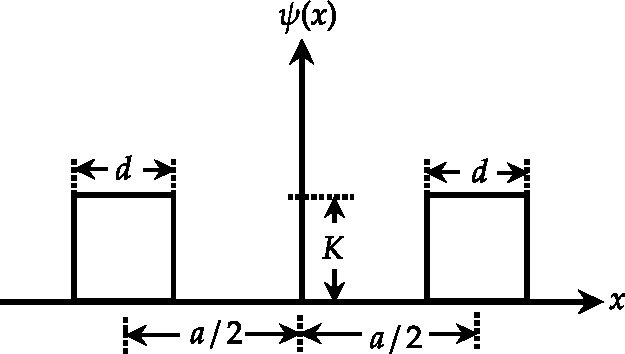
\includegraphics[height=3.6cm,width=6.3cm]{QM-3}
\end{figure}
Here $K$ is a constant, and $a>d$. The position uncertainty $(\Delta x)$ of the particle is
 \begin{tasks}(2)
	\task[\textbf{a.}]$\sqrt{\frac{a^{2}+3 d^{2}}{12}}$
	\task[\textbf{b.}] $\sqrt{\frac{3 a^{2}+d^{2}}{12}}$
	\task[\textbf{c.}]$\sqrt{\frac{d^{2}}{6}}$
	\task[\textbf{d.}] $\sqrt{\frac{d^{2}}{24}}$
\end{tasks}
\begin{answer}
So the correct answer is \textbf{Option (b)}
\end{answer}
\item A particle of mass $m$ is interact with potential which is given by $V(x)=-\lambda \delta(x)$ where $\lambda>0$ then which one of following is wrong statement about system?
 \begin{tasks}(2)
	\task[\textbf{a.}]There is only one bound state.
	\task[\textbf{b.}]The eigen function is continuous everywhere.
	\task[\textbf{c.}]The eigen function is differentiable every where
	\task[\textbf{d.}] The eigen function is square integrable.
\end{tasks}
\begin{answer}
	$$
	\begin{aligned}
	\psi(x)=\sqrt{\gamma} \exp -\gamma|x| \text { where } \gamma=\sqrt{\frac{-2 m E}{\hbar^{2}}} \text { where } 0<E
\end{aligned}
$$
So the correct answer is \textbf{Option (c)}
\end{answer}
\item Let $|n\rangle$ denote the energy eigenstates of a particle in a one-dimensional simple harmonic potential $V(x)=\frac{1}{2} m \omega^{2} x^{2}$. If the particle is initially prepared in the state $|\psi(t=0)\rangle=\sqrt{\frac{1}{2}}(|1\rangle+|2\rangle)$, the minimum time after which the oscillator will be found in the same state is
 \begin{tasks}(2)
	\task[\textbf{a.}]$3 \pi /(2 \omega)$
	\task[\textbf{b.}]$\pi / \omega$
	\task[\textbf{c.}]$\pi /(2 \omega)$
	\task[\textbf{d.}]$2 \pi / \omega$ 
\end{tasks}
\begin{answer}
	$$
	\begin{aligned}
	|\psi(t=0)\rangle&=\sqrt{\frac{1}{2}}(|1\rangle+|2\rangle)|\psi(t=t)\rangle=\sqrt{\frac{1}{2}}\left(|1\rangle e^{-\frac{3 i o t}{2}}+|2\rangle e^{-\frac{i 5 \omega t}{2}}\right)\\
	|\langle\psi(t) \mid \psi(0)\rangle|^{2}&=1 \Rightarrow\left|\frac{1}{2}\left(\exp -\frac{i 3 \omega t}{2}+\exp -\frac{5 i \omega t}{2}\right)\right|^{2}=1\\
	|1+\exp (-i \omega t)|^{2}&=4 \Rightarrow t=\frac{2 \pi}{\omega}
\end{aligned}
$$
So the correct answer is \textbf{Option (d)}
\end{answer}
\item If one dimension potential is given by $V(x)=\frac{1}{2} m \omega^{2} x^{2}$ (where $m$ and $\omega$ are constant).
If $\psi(x)=\sqrt{\frac{2}{3}} \phi_{0}(x)+i \sqrt{\frac{1}{3}} \phi_{1}(x)$, where $\phi_{0}$ and $\phi_{1}$ are ground state and first excited state of Hamiltonian operator, the expectation value of energy is given by
 \begin{tasks}(2)
	\task[\textbf{a.}]$-\frac{\hbar \omega}{6}$
	\task[\textbf{b.}]$\frac{5 \hbar \omega}{6}$
	\task[\textbf{c.}]$\frac{\hbar \omega}{6}$
	\task[\textbf{d.}] $\frac{4 \hbar \omega}{3}$
\end{tasks}
\begin{answer}
	$$
	\begin{aligned}
	\frac{2}{3} \cdot \frac{\hbar \omega}{2}+\frac{1}{3} \cdot \frac{3 \hbar \omega}{2}=\frac{5 \hbar \omega}{6}
\end{aligned}
$$
So the correct answer is \textbf{Option (b)}
\end{answer}
\item A quantum mechanical particle in a harmonic oscillator potential has the initial wave function $\psi_{0}(x)+\psi_{1}(x)$, where $\psi_{0}$ and $\psi_{1}$ are the real wavefunctions in the ground and first excited state of the harmonic oscillator. For convenience, we take $m=\hbar=\omega=1$ for the oscillator. What is the probability density of finding the particle at position $x$ and at time $t=\pi$ ?
 \begin{tasks}(2)
	\task[\textbf{a.}]$\left(\psi_{1}(x)-\psi_{0}(x)\right)^{2}$
	\task[\textbf{b.}]$\left(\psi_{1}(x)\right)^{2}-\left(\psi_{0}(x)\right)^{2}$
	\task[\textbf{c.}]$\left(\psi_{1}(x)+\psi_{0}(x)\right)^{2}$
	\task[\textbf{d.}] $\left(\psi_{1}(x)\right)^{2}+\left(\psi_{0}(x)\right)^{2}$
\end{tasks}
\begin{answer}
	$$
	\begin{aligned}
	\psi(x)&=\psi_{0}(x)+\psi_{1}(x) \Rightarrow \psi(x, t)=\psi_{0}(x) e^{-i} \frac{E_{0} t}{\hbar}+\psi_{1}(x) e^{-i} \frac{E_{1} t}{\hbar}\\
	&\text { Now probability density at time } t \text {, }\\
	|\psi(x, t)|^{2}&=\psi^{*}(x, t) \psi(x, t)=\left|\psi_{0}(x)\right|^{2}+\left|\psi_{1}(x)\right|^{2}+2 \operatorname{Re} \psi_{0}^{*}(x) \psi_{1}(x) \cos \left(E_{1}-E_{0}\right) \frac{t}{\hbar}\\
	 \text { Putting } t&=\pi\\
	|\psi(x, t)|^{2}&=\left|\psi_{0}(x)\right|^{2}+\left|\psi_{1}(x)\right|^{2}+2 \operatorname{Re} \psi_{0}^{*}(x) \psi_{1}(x) \cos \pi \quad\left[\because E_{1}-E_{0}=\hbar \omega=1\right]\\
	|\psi(x, t)|^{2}&=\left|\psi_{0}(x)\right|^{2}+\left|\psi_{1}(x)\right|^{2}-2 \operatorname{Re} \psi_{0}^{*}(x) \psi_{1}(x)=\left[\psi_{1}(x)-\psi_{0}(x)\right]^{2}
\end{aligned}
$$
So the correct answer is \textbf{Option (a)}
\end{answer}
\end{enumerate}